\documentclass[11pt]{article}
\usepackage[T1]{fontenc}
\usepackage[utf8]{inputenc}
\usepackage{mathptmx,courier}
\usepackage[margin=2.7cm]{geometry}
\usepackage{amsmath,amssymb,booktabs,array,graphicx,float}
\usepackage{setspace,microtype}
\usepackage[numbers,sort&compress]{natbib}
\usepackage[colorlinks=true,linkcolor=blue,citecolor=blue,urlcolor=blue]{hyperref}
\setstretch{1.18}
\raggedbottom
\AtBeginDocument{\lefthyphenmin=2\righthyphenmin=3}
\renewcommand{\topfraction}{0.9}
\renewcommand{\textfraction}{0.05}
\renewcommand{\floatpagefraction}{0.85}
\setlength{\emergencystretch}{2em}
\newcommand{\ind}{\mathbf{1}}
\newcommand{\equalcontribution}{Siyuan Tong and Yuechen Wang contributed equally to this work and share first authorship.}
\newcommand{\jointauthors}{\begin{minipage}{0.96\textwidth}\centering Siyuan Tong$^\dagger$ and Yuechen Wang$^\dagger$\\[0.3em]\small $^\dagger$\equalcontribution\end{minipage}}
\newcommand{\papertitle}{Separating coverage gains from error targeting in molecular prediction sets}
\hypersetup{pdftitle={Separating coverage gains from error targeting in molecular prediction sets},pdfauthor={Siyuan Tong and Yuechen Wang}}

\title{\papertitle}
\author{\begin{minipage}{0.96\textwidth}\centering
Siyuan Tong$^{1,*}$ and Yuechen Wang$^2$\\[0.3em]
\small $^1$Department of Artificial Intelligence, Faculty of Computer Science and Information Technology, University of Malaya, 50603 Kuala Lumpur, Malaysia\\
\small $^2$Faculty of Data Science, City University of Macau, Macau SAR, China\\
\small $^*$Corresponding author: \texttt{25064241@siswa.um.edu.my}
\end{minipage}}
\date{}
\begin{document}
\maketitle
\begin{abstract}
Expanding molecular prediction sets can improve coverage by deferring more compounds, without improving the selection of errors for deferral. We develop a class-budget comparison that separates these effects and an exact activation condition for weighted set expansion. The comparison holds the molecular predictor, eligible targets, and numbers of expanded baseline singletons in each predicted class fixed. We apply it to a two-view transport envelope across twelve Tox21 assays, three classical predictors, and fixed random and scaffold holdouts from four additional assay families; the complete experiment contains 960 predictor units. On the historical six-assay EPA panel, inactive-label protection increased mean minimum-class coverage from 83.74\% to 85.10\%, while operational deferral increased from 42.01\% to 44.02\% and macro correct-singleton yield decreased from 48.18\% to 46.57\%. Ranking the omitted label's probability reproduced the coverage gain at the same class-specific budget; the coverage difference was 0.000 percentage points (molecule-cluster bootstrap 95\% interval, $-0.028$ to $0.029$). Active-label protection passed both transport gates in all 30 primary cells but produced no additional deferrals. Across all twelve assays it added 21 compound--fit deferrals without recovering an erroneous inactive decision. The activation condition explains why gate passage need not change a prediction set, while a constant-query-weight result identifies when expansion reduces to probability ranking. These results provide a practical evaluation framework for distinguishing coverage purchased through deferral from additional error-targeting information under molecular distribution shift.
\end{abstract}
\noindent\textbf{Keywords:} molecular prediction; conformal prediction; distribution shift; selective prediction; deferral; class-specific coverage

\section{Introduction}
Molecular property prediction supports decisions about which compounds to advance, discard, or measure again. A binary prediction set makes the distinction explicit: a singleton selects one outcome, while a two-label set leaves the decision unresolved. Expanding singletons into two-label sets can protect measured outcomes that would otherwise be excluded. It also increases the number of compounds requiring further evidence. Evaluating this trade-off requires asking both how often a system covers the measured outcome and which decisions it withholds.

Conformal prediction constructs sets with coverage guarantees under specified sampling assumptions. Marginal coverage and class-conditional coverage answer different questions; Mondrian calibration addresses the latter under within-class exchangeability \citep{vovk2012}. Molecular collections often differ in composition and support, motivating methods that use unlabeled target compounds to estimate distribution shift. Weighted conformal prediction formalizes likelihood-ratio adjustment under covariate shift \citep{tibshirani2019}. CoDrug combines representation learning with density estimation \citep{codrug2023}, while KMM-CP uses kernel mean matching and selective support overlap \citep{kmm2026}. Their ability to restore coverage is a different question from their ability to make informative decisions at a given workload.

Selective classification has long studied the relation between error and abstention \citep{elyaniv2010}. For a prediction-set expansion, however, matching only total abstention can leave a further imbalance: methods may defer different proportions of original class-0 and class-1 decisions. This matters in molecular assays with uneven class frequencies and unequal costs of false-positive and false-negative decisions. Moreover, a Mondrian singleton need not be the probability argmax. Ranking uncertainty around probability 0.5 may therefore differ from ranking the probability of the particular label omitted by that singleton.

We use the transport-audited multi-view envelope (TAME) as a concrete case study. TAME adds a protected label when two weighted views agree, subject to transport diagnostics. Its historical label-0 version improved minimum-class coverage relative to a stacked Mondrian baseline. The interpretation depends on whether the selected deferrals contain more errors than an equally costly simple rule. We examine this directly by matching the expansion count within each original singleton class and ranking the probability of the omitted label.

The study makes three connected contributions. First, it provides a comparison design and an error--yield decomposition that separate expansion volume, predicted-class allocation, and error targeting. Second, an exact weighted-rank condition separates gate passage from actual label addition and identifies a setting in which expansion reduces to probability ranking. Third, a complete molecular experiment applies these diagnostics to the historical coverage gain, a prespecified active-label comparison, alternative predictors and scores, and four additional assay families. The contribution is the resulting explanation of when apparent coverage gains represent additional decision information.

\section{Methods}
\subsection{Molecular cohorts and experimental roles}
The Tox21 challenge supplies twelve nuclear-receptor and stress-response assays \citep{huang2016}. The source collection supplies model-fitting, stack-fitting, and calibration roles. The public leaderboard contains 296 structures and the final EPA collection 647 before structure standardization and overlap exclusions. The historical primary panel comprises NR-AhR, NR-ER, SR-ARE, SR-ATAD5, SR-MMP, and SR-p53, selected in the original development analysis by at least twenty positive labels. We retain this panel and report all twelve assays separately. EPA labels had been accessed in the earlier study, so the present EPA comparisons are retrospective.

The additional assay families are AMES mutagenicity, the standard hERG blockade dataset, drug-induced liver injury (DILI), and CYP2D6 inhibition from the Veith collection \citep{ames2012,herg2016,dili2015,veith2009}. Labels retain these endpoint-specific meanings. Tox21 activity is not a general toxicity diagnosis, and the CYP assay signal does not by itself resolve inhibition from substrate competition. Standardization uses RDKit 2026.03.4. Same-label duplicate structures are collapsed, and structures with conflicting binary labels are removed. The resulting AMES, hERG, DILI, and CYP2D6 source tables contain 7,255, 607, 474, and 13,083 structures, respectively.

Each additional dataset has a fixed random target split and a fixed scaffold target split, each approximately 20\% of the source table. Target counts are 1,451, 122, 95, and 2,617, respectively. Outer seeds are 43021 and 43022. Target selection uses structure or scaffold identity without outcome stratification. Five fits, seeds 311--315, reuse each fixed target cohort. These are within-dataset holdouts across additional endpoints. Supplementary Table S1 reports target, labeled-class, and calibration counts; acquisition and exclusion rules are specified in the archived data adapters.

\subsection{Predictors and prediction sets}
The shared-predictor comparison uses 2048-bit radius-two Morgan fingerprints. The historical source allocation is 60\% model fitting, 20\% stack fitting, and 20\% conformal calibration. The three predictors are logistic regression, a logistic stack over logistic regression/random forest/extra trees/Bernoulli naive Bayes, and an equal-logit combination. All uncertainty rules within a predictor use the same probabilities and eligible rows. Development fits use seeds 101--105 and EPA fits 211--215.

For candidate label $y\in\{0,1\}$ and fitted probability $p_y(x)$, the least-ambiguous-classification score is $s(x,y)=1-p_y(x)$. For $n_y$ observed class-$y$ calibration scores, the ordinary Mondrian threshold is order statistic $k_y=\lceil(n_y+1)(1-\alpha_y)\rceil$, or $+\infty$ when $k_y>n_y$. An empty calibration class also receives an infinite threshold. The candidate label selects the threshold. The set contains $y$ if $s(x,y)\le q_y$. The primary level is $\alpha_0=\alpha_1=0.10$; levels 0.05 and 0.20 and deterministic adaptive-prediction-set scores are sensitivities \citep{romano2020}.

We map $\{0\}$ to a negative/inactive decision, $\{1\}$ to a positive/active decision, and $\{0,1\}$ to deferral. Empty sets are repaired to the full set for all operational expansion comparisons; their raw frequency is retained separately. Let $S_0(x)$ denote this repaired baseline.

\subsection{Transport expansion and its activation condition}
TAME estimates target-to-calibration density ratios in two views: nine physicochemical descriptors and component/stack logits. Logistic domain-classifier odds are adjusted for domain sample sizes and clipped to $[0.05,20]$. A third fingerprint view is retained as a diagnostic comparator. Sample sizes, effective sample sizes, clipping, domain discrimination, and weighted mean discrepancy determine view eligibility. The fixed gates and their one-at-a-time sensitivities are in Supplementary Table S2.

For a given view $v$, positive calibration weights $w_{iv}$ and query weight $w_v(x)$ define the class distribution
\begin{equation}
 F_{v,x,y}=\frac{\sum_{i:Y_i=y} w_{iv}\delta_{s(X_i,y)}+w_v(x)\delta_{+\infty}}{W_{v,y}+w_v(x)},
 \qquad W_{v,y}=\sum_{i:Y_i=y}w_{iv}.
\end{equation}
Its $(1-\alpha_y)$ quantile gives the weighted threshold. A protected label omitted by $S_0(x)$ is added if both required views pass the gates and contain that label. Otherwise the baseline is retained. We distinguish historical protection of label 0 from the prespecified label-1 objective of reducing erroneous inactive decisions for active compounds.

Define the strict lower-score mass
\begin{equation}
 B_{v,y}(s)=\sum_{i:Y_i=y}w_{iv}\ind\{s(X_i,y)<s\}.
\end{equation}
The weighted set contains a finite candidate score $s=s(x,y)$ exactly when
\begin{equation}
 B_{v,y}(s)<(1-\alpha_y)\{W_{v,y}+w_v(x)\}. \label{eq:activation}
\end{equation}
Equivalently, the query weight must exceed $B_{v,y}(s)/(1-\alpha_y)-W_{v,y}$. The strict inequality accounts for ties at a quantile boundary. With no class-$y$ calibration observations it holds for every positive query weight, consistently with an infinite threshold. Supplementary Section S1 proves the condition and tests its boundary behavior against the executable quantile.

Equation \ref{eq:activation} yields three distinct checks: are the views eligible, do they add a label that the baseline omitted, and does that addition recover an erroneous decision? Gate passage alone does not imply either later event. This is an algebraic characterization of the expansion rule; coverage guarantees still require the relevant conformal assumptions.

If each view's query weight is constant across the target batch, its candidate threshold is constant. Under binary LAC, adding label 1 then selects an upper level set of $p_1(x)$ within baseline $\{0\}$ decisions. The two-view intersection uses the larger probability cutoff, and the union the smaller. At the resulting expansion count, ranking the omitted-label probability selects exactly the same set. Label-0 protection has the analogous result for $p_0(x)$ within baseline $\{1\}$. Query-varying weights are therefore necessary for a different ranking within this setting, although they need not improve error targeting.

\subsection{Matching budgets and decomposing gains}
For an expansion $S$ of $S_0$, define
\begin{equation}
 m_c=\sum_{i\in\mathcal E}\ind\{S_0(x_i)=\{c\},\,|S(x_i)|=2\},\qquad c\in\{0,1\},
\end{equation}
where $\mathcal E$ includes every eligible target, including those without an observed assay outcome. Each comparator expands exactly $m_0$ and $m_1$ decisions, ranked within their original singleton classes. The primary comparator ranks $p_{1-c}(x)$, the probability of the omitted label. Secondary rankings use uncertainty around 0.5, lower maximum training-set Tanimoto similarity, and fixed seeded random priorities. Stable molecule identifiers resolve ranking ties. Target outcomes are absent from ranking and budget selection.

Within one baseline class-$c$ pool, let $R$ count expanded labeled decisions whose true class is $1-c$, and $L$ count those whose true class is $c$. For the fixed labeled-class denominators $N_y$,
\begin{equation}
 \Delta C_{1-c}=R/N_{1-c},\qquad
 \Delta\mathrm{CSY}_c=-L/N_c,\qquad R+L=m_c^{\mathrm{obs}}.
\end{equation}
Here $C_y$ is class coverage and $\mathrm{CSY}_y$ is correct-singleton yield. The observed-label expansion count $m_c^{\mathrm{obs}}$ may differ from the operational count $m_c$ when outcomes are missing. At equal observed-label budgets, greater error recovery necessarily preserves more correct singletons in the original class. At equal operational budgets, the observed-budget difference must also be included. Supplementary Section S1 gives this correction for two competing rules.

We report minimum-class coverage $C_{\min}=\min(C_0,C_1)$, macro correct-singleton yield $\mathrm{MacroCSY}=(\mathrm{CSY}_0+\mathrm{CSY}_1)/2$, false-inactive exposure $E_1=\Pr\{S=\{0\}\mid Y=1\}$, false-active exposure $E_0=\Pr\{S=\{1\}\mid Y=0\}$, and decision yield. Operational deferral uses all eligible targets; coverage and errors use observed labels. Empty denominators remain undefined.

\subsection{Comparisons and inference}
The fixed primary contrast compares active-label TAME with its omitted-label-probability comparator for $E_1$, using the stack, LAC, $\alpha=0.10$, and the historical six assays. The historical label-0 comparison explains the earlier coverage gain. The full matrix includes the three classical predictors, marginal/Mondrian LAC and APS, weighted variants, protected-label variants, single-view and union rules, ungated rules, fourteen gate sensitivities, and five gated plus five ungated query-weight permutations. Each expansion variant receives its own class-budget-matched probability comparator. Fixed workload curves use fractions 0, 0.10, 0.25, 0.50, 0.75, and 1 of the baseline singleton pool.

The end-to-end reference systems are independent paper-based CoDrug and KMM-CP implementations with AttentiveFP predictors. CoDrug includes its energy penalty, auxiliary molecular pool, and logit-space density estimates. Both printed and prespecified swapped energy-margin settings are retained. KMM-CP includes ordinary and selective kernel mean matching, bandwidth selection, and refitting after target selection. Candidate-label and literal predicted-group threshold interpretations are reported separately. Unselected targets defer in the full-cohort comparison. These systems use their own predictors and native workloads; their recorded settings and all ten configurations appear in Supplementary Section S3 and Table S4.

The complete experiment completed 960 predictor units: 360 development, 360 EPA, 120 random holdout, and 120 scaffold holdout. Of these, 480 use classical predictors and 480 use neural reference systems. Alpha levels and post-prediction variants reuse a unit's probabilities. Metrics are computed within assay--seed cells and then averaged equally over the declared panel. Bootstrap intervals resample molecular/structure identities jointly across assays and methods while retaining every seed prediction, using 2,000 replicates and seed 44021. The interval estimand is the fixed-panel mean; training seeds do not add independent molecules. Secondary intervals are pointwise exploratory.

Synthetic mechanisms with thirty replicates each examine no shift, overlapping covariate shift, support loss, and changed $Y\mid X$ with identical observable covariates. These analyses are reported separately in Supplementary Section S5.
\section{Results}
\subsection{The historical coverage gain is reproduced at matched cost}
On the historical six-assay EPA panel, label-0 TAME increased mean minimum-class coverage from 83.739\% to 85.104\%, a gain of 1.3649 percentage points. Operational deferral increased by 2.0164 points, from 42.007\% to 44.023\%, and MacroCSY fell by 1.6067 points, from 48.179\% to 46.572\% (Table \ref{tab:historical}). The expansion recovered some false-active decisions while withholding additional correct positive singletons.

The class-budget-matched omitted-label-probability rule reached the same mean minimum-class coverage, MacroCSY, and deferral. The TAME-minus-probability difference in minimum coverage was 0.0000 points, with a molecule-cluster bootstrap 95\% interval of $[-0.0279,0.0287]$ points. The nondegenerate interval is consistent with differences among individual decisions despite identical aggregate means. This result attributes the historical gain to an attainable error--deferral trade-off rather than additional demonstrated ranking information from transport.

\begin{table}[htbp]\centering\small
\caption{Historical six-assay EPA means with the stack and $\alpha=0.10$. Entries are percentages. The four simple ranking rules use the exact label-0 TAME class budgets. The last row uses the separate active-label objective. $E_0$ is false-active exposure.}\label{tab:historical}
\begin{tabular}{lrrrr}\toprule
Rule & $C_{\min}$ & $E_0$ & MacroCSY & Deferral \\
\midrule
Mondrian LAC baseline & 83.74 & 14.64 & 48.18 & 42.01 \\
TAME, label 0 & 85.10 & 12.93 & 46.57 & 44.02 \\
Omitted-label probability & 85.10 & 12.93 & 46.57 & 44.02 \\
Probability uncertainty & 84.75 & 13.44 & 44.61 & 44.02 \\
Chemical similarity & 84.83 & 13.21 & 45.65 & 44.02 \\
Seeded random selection & 84.87 & 13.24 & 45.34 & 44.02 \\
TAME, label 1 & 83.74 & 14.64 & 48.18 & 42.01 \\
\bottomrule\end{tabular}

\end{table}

The choice of simple comparator was consequential. At the same operational budget, omitted-label ranking obtained 85.10\% minimum-class coverage and 46.57\% MacroCSY, compared with 84.75\% and 44.61\% for probability uncertainty. Similarity and random rankings also gave lower descriptive coverage and yield than omitted-label ranking (Table \ref{tab:historical}). Thus comparison against generic uncertainty alone would overstate the need for transport information. Figure \ref{fig:assays} displays the assay-level results, including the six assays outside the historical panel.

\begin{figure}[htbp]\centering
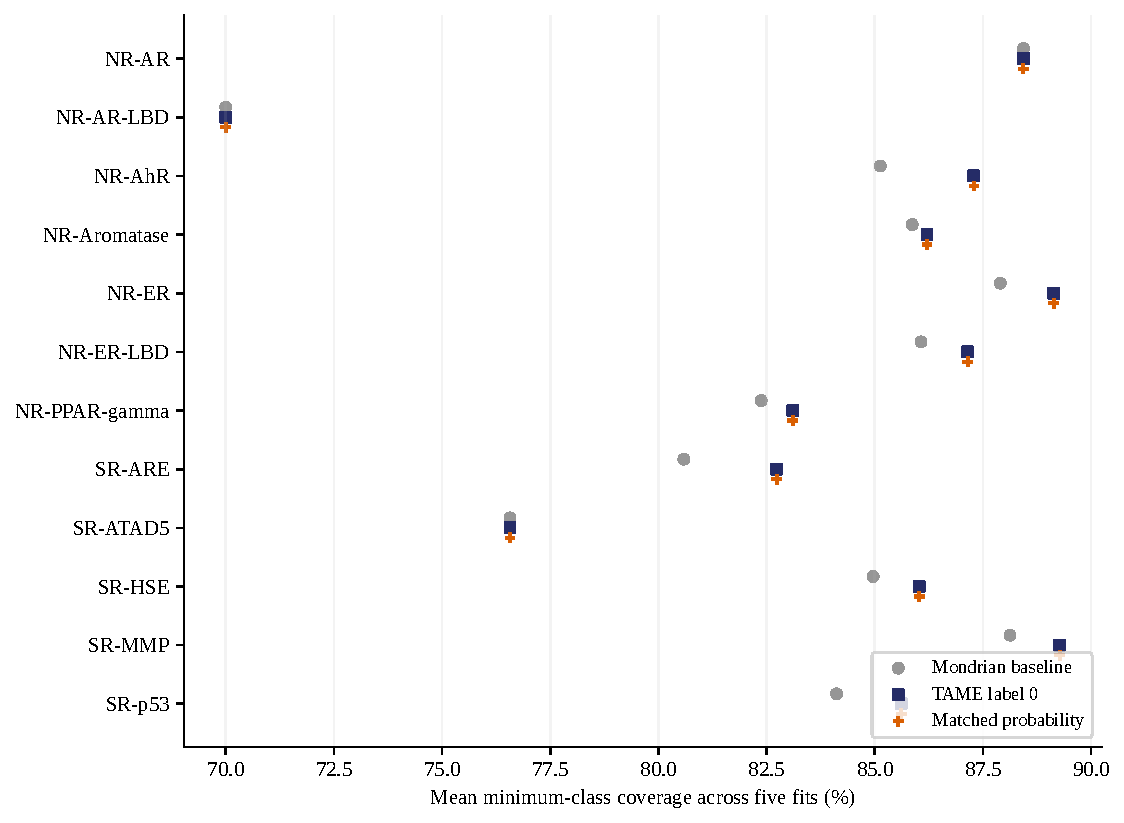
\includegraphics[width=.86\textwidth]{figures/assay_coverage.pdf}
\caption{Assay-level EPA coverage for the stack at $\alpha=0.10$, averaged over five fits. Markers are vertically offset for legibility. Aggregate agreement does not imply identical compound-level selections.}\label{fig:assays}
\end{figure}

\subsection{Gate passage and active-label expansion separate}
In the fixed active-label primary comparison, both transport views passed in every one of the 30 assay--seed cells. Nevertheless, the expansion count was zero in all 30. TAME, its matched comparators, and repaired Mondrian therefore produced the same primary decisions: false-inactive exposure was 10.532\%, minimum-class coverage 83.739\%, and operational deferral 42.007\%. The reported zero difference and degenerate bootstrap interval arise from no intervention in this panel; they do not measure the relative quality of two nonempty rankings.

Across all twelve EPA assays, both views passed in all 180 classical predictor cells. For the stacked predictor, active-label TAME added 21 compound--fit deferrals, concentrated in NR-AR and NR-AR-LBD. Seven were selected only by TAME and seven only by the matched probability rule. Neither rule recovered a false-inactive decision among these additions. Because the sums span fitted repetitions, they count repeated decisions rather than independent compounds (Table \ref{tab:activation}).

\begin{table}[htbp]\centering\small
\caption{Active-label mechanism counts at $\alpha=0.10$ with the stack. Pass requires both views. Added counts are equal for TAME (A) and matched probability (P); A-only/P-only denotes discordant selections. Rescued lists erroneous inactive decisions recovered by A/P. Counts sum over fit seeds; the two EPA rows overlap.}\label{tab:activation}
\begin{tabular}{lrrrr}\toprule
Setting & Pass / cells & Added & A-only / P-only & Rescued \\
\midrule
EPA, historical six & 30 / 30 & 0 & 0 / 0 & 0 / 0 \\
EPA, all twelve & 60 / 60 & 21 & 7 / 7 & 0 / 0 \\
AMES / random & 5 / 5 & 0 & 0 / 0 & 0 / 0 \\
CYP2D6 / random & 5 / 5 & 0 & 0 / 0 & 0 / 0 \\
DILI / random & 0 / 5 & 0 & 0 / 0 & 0 / 0 \\
hERG / random & 0 / 5 & 0 & 0 / 0 & 0 / 0 \\
AMES / scaffold & 5 / 5 & 0 & 0 / 0 & 0 / 0 \\
CYP2D6 / scaffold & 5 / 5 & 19 & 0 / 0 & 1 / 1 \\
DILI / scaffold & 0 / 5 & 0 & 0 / 0 & 0 / 0 \\
hERG / scaffold & 0 / 5 & 0 & 0 / 0 & 0 / 0 \\
\bottomrule\end{tabular}

\end{table}

\subsection{Additional assay families distinguish fallback from nonactivation}
AMES and CYP2D6 passed both transport gates in every shared-predictor fit under both split regimes. hERG failed the 100-calibration-observation threshold. DILI also had fewer than 100 target structures. Their active-label rules consequently retained the baseline. These are different reasons for observing a zero matched effect.

For the stack, all four random-holdout tasks had zero additional deferrals. The scaffold CYP2D6 analysis added 19 compound--fit deferrals, identical under TAME and matched probability; both recovered one false-inactive decision. Its false-inactive exposure decreased from 10.410\% to 10.369\%, with deferral increasing from 34.375\% to 34.520\%. The remaining stacked scaffold tasks added no deferrals.

Across all 24 endpoint/split/predictor active-label comparisons, 23 had zero error differences. The remaining CYP2D6 random-split equal-logit contrast was $-0.0418$ points, with a pointwise interval of $[-0.1330,0.0000]$. The experiment therefore distinguishes small-sample fallback, eligible but inactive expansion, and a small nonempty expansion reproduced by the simple ranking rule.

\subsection{Predictor, workload, and reference-system comparisons}
The underlying predictor changes the trade-off even before transport expansion. On the historical panel, ordinary equal-logit Mondrian had 84.82\% minimum-class coverage and 46.70\% MacroCSY at 44.37\% deferral; logistic Mondrian had 84.84\%, 43.51\%, and 47.58\%, respectively. The stack had lower minimum coverage but higher MacroCSY and fewer deferrals (Supplementary Table S3). Comparing one column could conceal these differences.

The fixed-workload curves show how coverage can rise as additional decisions are withheld (Figure \ref{fig:workload}). At its native operating point, deterministic Mondrian APS reached 91.38\% minimum-class coverage and zero false-inactive exposure, while deferring 89.68\% of eligible targets and retaining 9.28\% MacroCSY. Its apparent coverage advantage is accompanied by a large reduction in informative decisions.

The neural reference systems likewise occupied different operating points. The swapped-margin CoDrug candidate-class variant gave 10.93\% false-inactive exposure at 36.58\% deferral and 52.97\% MacroCSY. Selective KMM with candidate-label thresholds gave 7.67\% false-inactive exposure at 52.79\% deferral and 36.27\% MacroCSY. All ten declared reference configurations, including the printed-margin CoDrug and predicted-group KMM interpretations, appear in Supplementary Table S4. These complete-system comparisons describe the trade-offs of different predictors and uncertainty rules.

\begin{figure}[htbp]\centering
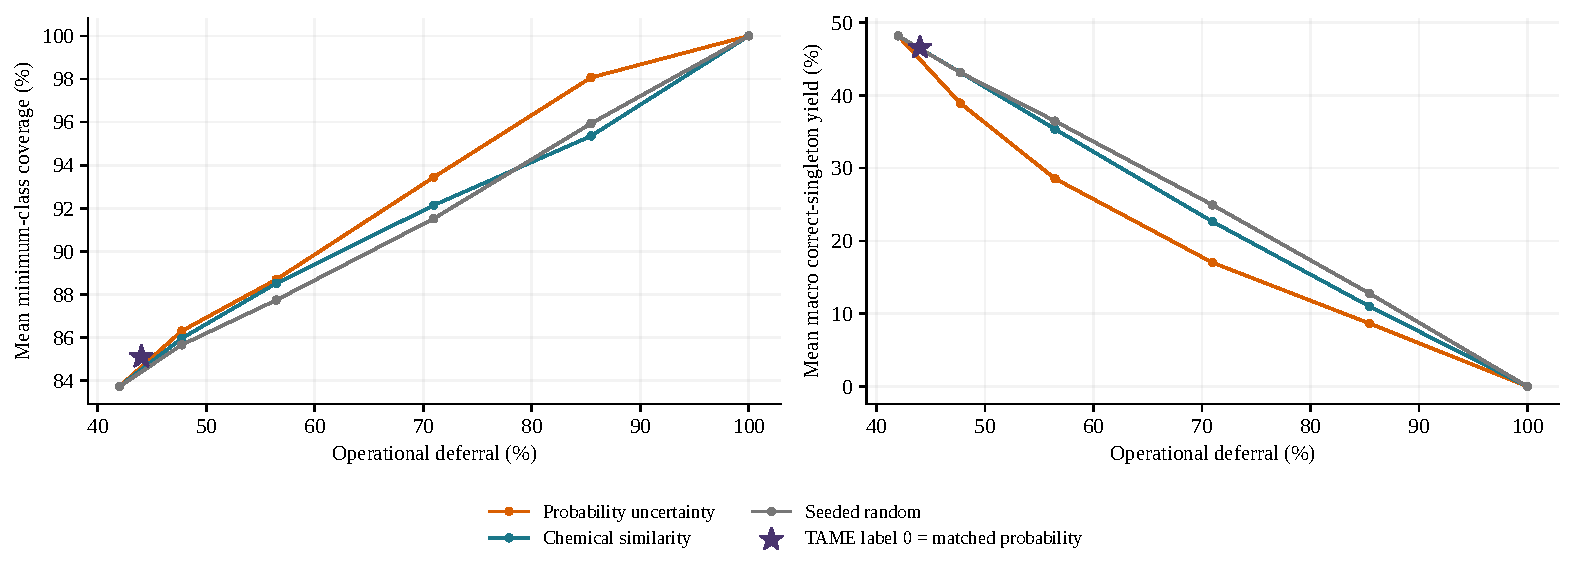
\includegraphics[width=\textwidth]{figures/workload_tradeoff.pdf}
\caption{Coverage and correct-singleton yield across fixed additional-deferral fractions on the historical EPA panel. The star marks the label-0 TAME and matched-probability point. They share these aggregate coordinates. Curves use uncertainty, similarity, or random ranking over the baseline singleton pool; they describe workload trade-offs rather than class-budget-matched effects at every point.}\label{fig:workload}
\end{figure}

\subsection{Ablations localize the absence of added targeting information}
Removing gates did not activate the stack's primary active-label expansion. A physicochemical-only view or view union added sixteen decisions in one primary assay--seed cell; their own-budget error difference was $-0.0952$ points, with an interval of $[-0.3030,0.0000]$. Across 280 declared own-budget ablation and query-alignment contrasts, no pointwise error interval excluded zero. The five gated and five ungated query-weight permutations each produced zero primary-panel budget, making that panel uninformative about the value of query-specific alignment.

In the synthetic paired no-shift and changed-conditional scenarios, all thirty pairs shared identical prediction and transport-diagnostic inputs. Active-label TAME nevertheless had mean class-1 coverage of 90.36\% and 39.74\%, respectively, with the same 30.30\% deferral. This mechanism check illustrates why diagnostics based only on the observed covariates cannot identify a changed conditional outcome law.

\section{Discussion}
The main empirical finding is that the historical coverage improvement survives recomputation but loses its interpretation as extra transport-based error targeting. An omitted-label-probability rule reproduces the 1.3649-point minimum-coverage gain at the same predicted-class budget. The framework makes this distinction measurable without changing the predictor or using target outcomes to rank compounds. It also shows why the strongest relevant simple comparator depends on the decision being deferred: a rule tailored to the omitted label can outperform generic probability uncertainty at identical cost.

The activation condition explains a second issue that aggregate accuracy tables obscure. A view can satisfy every diagnostic gate and still fail to add the protected label to any baseline singleton. In that case, zero matched differences reflect an unused intervention. Conversely, an expansion can occur without rescuing an error, as in the all-twelve-assay active-label result. Reporting gate eligibility, additions, discordant selections, and recovered errors in sequence connects the mathematical rule to the actual decisions.

The constant-query-weight result clarifies what transport weighting can contribute. With fixed query mass, changing source weights or a cell-level gate can move the probability threshold and hence the budget, but cannot change the within-pool ordering. Query-dependent thresholds can depart from that ordering; useful departures must concentrate errors more effectively at equal cost. The molecular results offer a direct test of this distinction, while leaving room for other predictors, shifts, and density estimators to produce different outcomes.

The scope of the evidence is a fixed collection of assays and molecular cohorts. Repeated fits quantify model variation but reuse compounds; the shared-structure bootstrap preserves this dependence. The additional families supply random/scaffold holdout checks, with visible small-sample fallback in hERG and DILI. Estimated and clipped ratios also differ from known likelihood ratios under exact covariate shift. These distinctions define what the reported comparisons estimate.

For molecular screening, the useful output is a joint account of recovered errors, surrendered correct decisions, and operational workload. A coverage gain can be scientifically informative even when a complex rule does not win: here it identifies a reproducible, simpler route to the same observed trade-off and provides an explicit test for when a transport-based expansion contributes information beyond that route.

\section{Conclusion}
Class-budget matching and an exact activation condition separate the cost and targeting components of molecular prediction-set expansion. In the evaluated TAME study, a simple omitted-label-probability ranking reproduced the historical coverage gain, while the prespecified active-label expansion was inactive on the primary panel. Reporting eligibility, intervention, and error recovery together gives a more informative assessment of molecular uncertainty procedures than coverage alone.

\section*{Data and code availability}
The data adapters, experiment suite, frozen aggregate inputs, manuscript sources, and rebuilding scripts are available in the \href{https://github.com/DCarchimonde/aidd-paper-factory/tree/paper2-tame-resubmission-20261112/paper2_latex/resubmission_20261112}{versioned project directory}. The complete numerical supplement retains all returned cell metrics, panel metrics, and paired contrasts. The manuscript rebuilding script operates on frozen aggregates; retraining and molecule-level inference use the experiment suite and its full exports.
\section*{Declaration of competing interest}
The authors declare no competing interests.
\section*{Funding}
The authors received no specific funding for this work.
\section*{CRediT authorship contribution statement}
Siyuan Tong: Conceptualization, Methodology, Software, Validation, Formal analysis, Investigation, Data curation, Visualization, Writing -- original draft, Writing -- review \& editing. Yuechen Wang: Methodology, Validation, Writing -- review \& editing.
\section*{Declaration of generative AI and AI-assisted technologies}
OpenAI ChatGPT was used for language editing, manuscript organization, LaTeX formatting, code assistance, and preparation of reproducibility materials. The authors are responsible for the content of the submitted manuscript.

\begin{thebibliography}{99}
\raggedright
\interlinepenalty=10000
\bibitem{vovk2012} V. Vovk, Conditional validity of inductive conformal predictors, Proceedings of Machine Learning Research 25 (2012) 475--490. \url{https://proceedings.mlr.press/v25/vovk12.html}.
\bibitem{tibshirani2019} R. J. Tibshirani, R. F. Barber, E. J. Cand\`es, A. Ramdas, Conformal prediction under covariate shift, Advances in Neural Information Processing Systems 32 (2019). \url{https://proceedings.neurips.cc/paper/2019/hash/8fb21ee7a2207526da55a679f0332de2-Abstract.html}.
\bibitem{codrug2023} S. Laghuvarapu, Z. Lin, J. Sun, CoDrug: Conformal drug property prediction with density estimation under covariate shift, Advances in Neural Information Processing Systems 36 (2023). \url{https://proceedings.neurips.cc/paper_files/paper/2023/hash/7691484a7a35d5e2742279c1d926b778-Abstract-Conference.html}.
\bibitem{kmm2026} S. Laghuvarapu, R. Deb, J. Sun, KMM-CP: Practical conformal prediction under covariate shift via selective kernel mean matching, Proceedings of Machine Learning Research 337 (2026) 3237--3261. \url{https://proceedings.mlr.press/v337/laghuvarapu26a.html}.
\bibitem{romano2020} Y. Romano, M. Sesia, E. Cand\`es, Classification with valid and adaptive coverage, Advances in Neural Information Processing Systems 33 (2020). \url{https://proceedings.neurips.cc/paper_files/paper/2020/hash/244edd7e85dc81602b7615cd705545f5-Abstract.html}.
\bibitem{huang2016} R. Huang, M. Xia, D.-T. Nguyen, T. Zhao, S. Sakamuru, J. Zhao, S. A. Shahane, A. Rossoshek, A. Simeonov, Tox21Challenge to build predictive models of nuclear receptor and stress response pathways as mediated by exposure to environmental chemicals and drugs, Frontiers in Environmental Science 3 (2016) 85. \url{https://doi.org/10.3389/fenvs.2015.00085}.
\bibitem{ames2012} C. Xu et al., In silico prediction of chemical Ames mutagenicity, Journal of Chemical Information and Modeling 52 (2012) 2840--2847. \url{https://doi.org/10.1021/ci300400a}.
\bibitem{herg2016} S. Wang et al., ADMET evaluation in drug discovery. 16. Predicting hERG blockers by combining multiple pharmacophores and machine learning approaches, Molecular Pharmaceutics 13 (2016) 2855--2866. \url{https://doi.org/10.1021/acs.molpharmaceut.6b00471}.
\bibitem{dili2015} Y. Xu et al., Deep learning for drug-induced liver injury, Journal of Chemical Information and Modeling 55 (2015) 2085--2093. \url{https://doi.org/10.1021/acs.jcim.5b00238}.
\bibitem{veith2009} H. Veith et al., Comprehensive characterization of cytochrome P450 isozyme selectivity across chemical libraries, Nature Biotechnology 27 (2009) 1050--1055. \url{https://doi.org/10.1038/nbt.1581}.
\bibitem{elyaniv2010} R. El-Yaniv, Y. Wiener, On the foundations of noise-free selective classification, Journal of Machine Learning Research 11 (2010) 1605--1641. \url{https://www.jmlr.org/papers/v11/el-yaniv10a.html}.
\end{thebibliography}

\end{document}
